\documentclass[oneside,openright,titlepage,numbers=noenddot,headinclude,
                footinclude=true,cleardoublepage=empty,
                BCOR=5mm,paper=a4,fontsize=11pt]{scrbook} 

\input{classicthesis-config}

\cfoot{\pagemark}

\begin{document}

\frenchspacing % Reduces space after periods to make text more compact
\raggedbottom % Makes all pages the height of the text on that page

\pagenumbering{roman} 
\pagestyle{plain}

\begin{titlepage}

%\begin{addmargin}[1cm]{3cm}
\begin{center}
\large

\hfill
\vfill

\begingroup
\color{Maroon}\spacedallcaps{\myTitle} \\ \bigskip % Thesis title
\endgroup

\spacedlowsmallcaps{\myNameA} \\% Your name
%\spacedlowsmallcaps{\myCodeA} \\ 

\vfill


\includegraphics[width=3cm]{images/logo} \\ \medskip % Picture

%\mySubtitle \\ \medskip % Thesis subtitle
%\myDegree \\
\myDepartment \\
\myFaculty \\
\myUni \\ \bigskip

\myTime\ %-- \myVersion  Time and version

\vfill

\end{center}
%\end{addmargin}

\end{titlepage}

\clearpage\pagestyle{scrheadings}
\clearpage\include{Chapters/Contents}
\pagenumbering{arabic} 
\clearpage\chapter{Introduction}


Actually the video devices capture a lot amount of information of some real world scene for processing in computing systems. With increasing of information, is necessary  to develop compression techniques for representing the video information with the lowest possible amount of bits for facilitating the storing and transmission. This advancements also have increased the requirements for video format as 4k(3840 $\times$ 2160px) and 8k(7680 $\times$ 4320px) for resolution, 10 bit depth and 50-60 for frame rate. Moreover, the advancement of technologies in the cloud for storing and computation, has prompted the use of services that use videos as streaming, video conference, IPTV among others, which has generated a significant increase in traffic of video over networks, in special for mobile applications, as can be seen in Fig. \ref{fig:vni}.

\begin{figure}[!h]
\centering
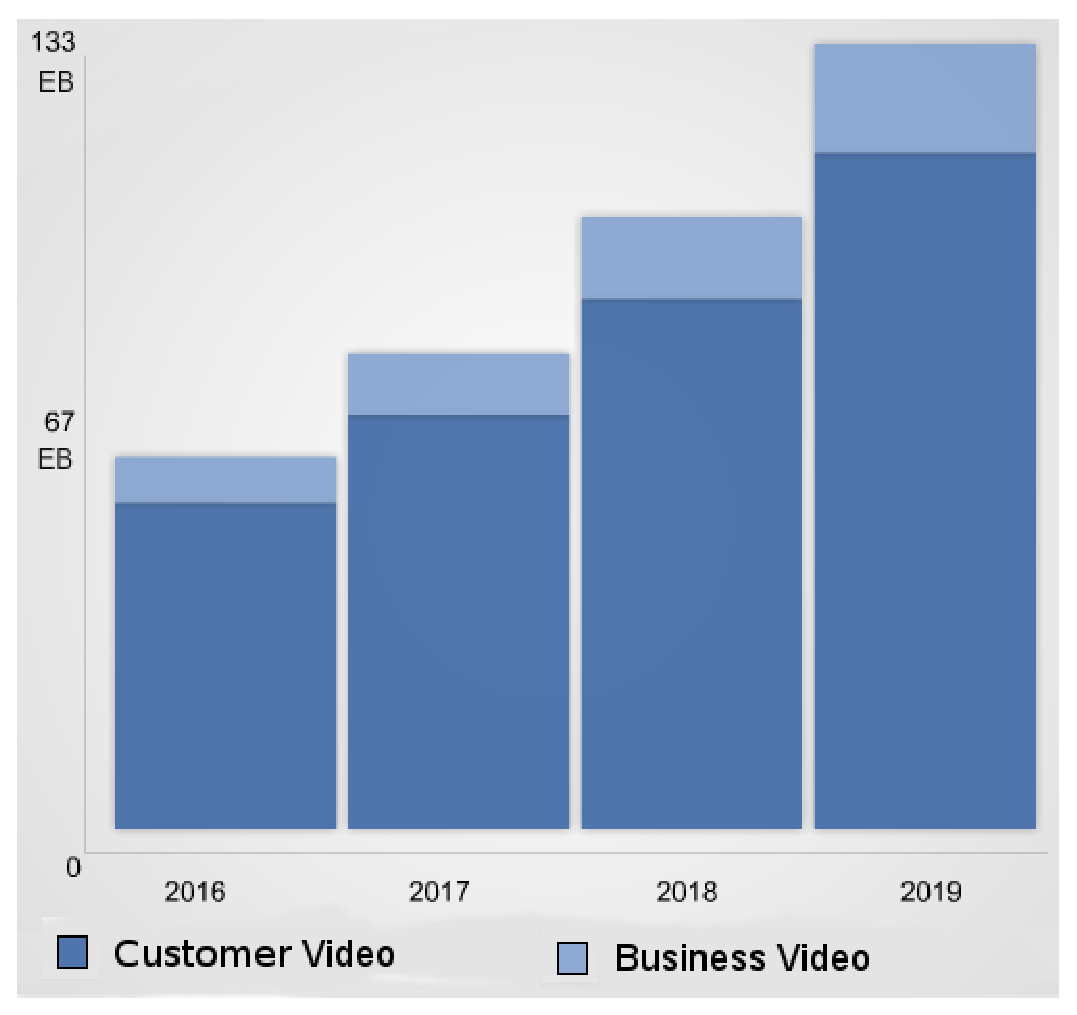
\includegraphics[width=0.4\textwidth]{images/vni.eps}
\caption[Estimated future global IP traffic growth for Video]{Estimated future global IP traffic growth for Video \scriptsize{Source: Cisco VNI Forecast}} 
\label{fig:vni}
\end{figure}

Video compression standards as MPEG4, H.264, VP9, HEVC among others have an important role in the transferring of video information through the cloud, looking with each generation of video encoders, increasingly reduce the bit rate. Conventional video encoders exploiting the correlation spatial and temporal between neighbour video frames. Instead of conventional video encoders, Compressive Sensing has emerged as a approach for simplifying the signal representation taking advantage of the sparse property of video signal which means that most of the signal coefficients are zero. Compressive sensing using a small number of sample for reconstruct a signal resolving a $\ell_p$- norm minimization problem using a trained dictionary of samples.\\

The main aim of video coding is to improve the coding efficiency, reducing the bit-rate for representing a video preserving a high level of quality with a maximum delay and complexity permitted. The complexity and bit-rate has been a important condition for video coding mainly in mobile applications due to processing and bandwidth limitations in the devices. Although cloud computing is a alternative for processing in devices with poor-resources, the latency is high. Fog Computing arise as a alternative, inside of cloud computing, for reducing the latency using the edge of the network for processing. \\

This project presents a proposal for video coding through the cloud network using compressive sensing to reduce the bit-rate. Dictionary learning process and sparse representation of the signal are performed in the fog network and directed toward the cloud. Dictionary and sparse vector are transferred for reconstruct the video  in the end-user side.

\section{Problem Statement}

Nowadays, the video services in the cloud have increased significantly thanks to popularity of applications in video-on-demand, broadcasting, live streaming, internet and mobile network video, video chat, telepresence systems and video conferencing. The evolution of this services create a stronger needs in terms of transmission bandwidth and processing for video, specially for High Definition (HD) content as 1080p, and the emerged beyond-HD content as 4k and with 8k. This video content required a greater amount of bits for represent it with a quality level acceptable. As an example, Table \ref{fig:youtube} shows the bit rates necessary for representing a live stream video of Youtube with a specific resolution using H.264 encoder. 

\begin{table}[!h]
\centering
\begin{tabular}{|c|c|c|}
\hline
\textbf{Resolution} & \textbf{Min bit rate (Kbps)} & \textbf{Max bit rate (Kbps)} \\
\hline
2560$\times$1440$@$60 & 9000 & 18000 \\
\hline
2560$\times$1440$@$30 &  6000 & 13000  \\
\hline
1920$\times$1080$@$60 & 4500 & 9000\\
\hline
1920$\times$1080 & 3000 & 6000 \\
\hline
\end{tabular}
\caption[Bit rates requirements for some resolutions in Live Stream Video of Youtube]{Bit rates requirements for some resolutions in Live Stream Video of Youtube \scriptsize{Source: \url{https://support.google.com/youtube/answer/2853702}}}
\label{fig:youtube}
\end{table}

In addition to high bit rates requirements, in some regions there are limitations on  network bandwidth, for example, Latin America has a internet connectivity speed of 7,26 Mbps on average while for mobile networks has a lower speed to 4 Mbps on average \cite{cepal}. High bit rates and network bandwidth limitation involve continuous efforts to maximise the coding efficiency, reducing the bit rates considering aspects as data loss and the computational resources in this process. Another feature to consider in video cloud applications that require high use of bandwidth is the delay between the cloud provider and end devices. The distance and shared nature of the cloud makes the data transmission susceptible to multiple kinds of delay which affect the user experience. Also the increase tendency of devices connected to internet with Internet of Things (IoT) makes the problem even more relevant. \\


Conventional Video encoders, as VP9, MPEG4 and H.26x, exploits the spatial and temporal redundancy, also applying an entropy coding and quantization process to improve the coding efficiency. This encoders have been  widely deployed and the three main process have been widely development, for this reason in necessary seek and adapt to the convectional video encoders other strategies for encoding process that can maximise the compression capability. 


\section{Objectives}
\subsection{General Objective}
Reduce the bit rates for representing a video in high definition based compressive sensing techniques using  fog computing.
\subsection{Specific Objectives}
\begin{itemize}
\item Evaluate different strategies for training learning in sparse representation based on video samples patches.
\item Define a scheme for video coding using compressive sensing based on the dictionary trained.
\item Design a framework for compressed video sensing based on the fog computing. 
\item Implements the proposed design for compressed video sensing.
\item Evaluate and compare the implemented model in terms of coding efficiency and delay using different video sequences.
\end{itemize}

\section{Project Scope}

The purpose of this project is focused on reducing the bit rates in the process of video coding using compressive sensing and the fundamentals of cloud computing. Based on the video coding principles, a video coding have two main applications: the encoder and the decoder, for this reason the designed scheme will have this elements. In the project will be used in existing algorithms in the literature for training the dictionary for sparse representation, the purpose of the project is not to design a new training algorithm. In addition, the project will be focused in high definition content therefore test videos sequences should be   high definition content.


\clearpage\chapter{Theoretical Background}

\section{Cloud Computing}
Cloud computing refers to the hardware, systems software, and applications delivered as services over the Internet \cite{cloud}. Cloud computing have services from a simple web services to data centers. Hardware for cloud computing can to consist of thousands of individual \emph{computing nodes} with their corresponding networking and storage subsystems, power distribution and conditioning equipment, and extensive cooling systems. Software for cloud computing can to consist of operative system in virtual machines, web applications and web services. 

Cloud computing have three deployment models: \emph{public, private} and \emph{hybrid}, and cloud services models can be grouped three categories:
\begin{itemize}
  \item Infraestructure as a Service(IaaS): providers offer computer power and   storage such as processors, virtual machines, data centers, serves, among others.
  \item Platform as a service(PaaS): providers offer the tools for developing applications such as operative systems, programming languages environments, databases among others.
  \item Software as a Service(SaaS): providers offer access to applications and databases.
\end{itemize}  

Figure \ref{cloud_services} show the stack estructure for cloud services.

\begin{figure}[!h]
\centering
\includegraphics[width=0.5\textwidth]{images/cloud_services}
\caption[Cloud computing service models]{Cloud computing service models \\
\scriptsize{\textbf{Source:} \url{http://www.ibm.com/developerworks/websphere/techjournal/1206_dejesus/1206_dejesus.html}}}
\label{cloud_services}
\end{figure}

\subsection{Virtualisation}

Virtualisation are a important component for cloud computing to decoupled the operative system of the physical infrastructure for adding flexibility. Virtualisation allows rapid deployment, reduce space and energy costs thanks to in a server can be running multiple operative systems. The main aim of virtualisation technologies 
is to hide the physical characteristics of computing resources from the way in which other systems, applications, or end users interact with those resources \cite{virtualization}. Hardware platform, operative system, networks and storage devices can be virtualised. 

\subsubsection{Virtual Machines}
A Virtual Machine(VM) is an instance of the physical machine and gave users the illusion of accessing the physical machine directly \cite{virtualization}. VMs are created and executed in a host machine by Virtual Machine Monitor or Hypervisor. The VMs can run legacy applications requiring an older platform and/or OS and run isolated of the underlying system. Also, it can create a single system image starting from an heterogeneous collection of machines, and can be performed faster job migration within different virtual machines running on the same hardware. These characteristics have led to the use of virtual machines for cloud computing. 

\subsubsection{Network Function Virtualisation}
The Network Function Virtualisation(NFV) involves the implementation of network functions in software that can run on a range of industry standard server hardware, and that can be moved to, or instantiated in, various locations in the network as required, without the need for installation of new equipment \cite{nfv}. European Telecommunications Standards Institute (ETSI) define a NFV framework \cite{nfv_framework} with three main working domains like is showed in figure \ref{nfv_framework}. 


\begin{figure}[!h]
\centering
\includegraphics[width=0.5\textwidth]{images/nfv_framework}
\caption[Network Function Virtualisation Framework]{Network Function Virtualisation Framework \\
\scriptsize{\textbf{Source:} Software-Defined Network Function
Virtualisation: A Survey - Figure 1}}
\label{nfv_framework}
\end{figure}

The \emph{Virtualised Network Functions} (VNF) are the software implementation of a network function, \emph{NFV Infrastructure} (NFVI) including the diversity of physical resources and \emph{NFV Management and Orchestration} which covers the orchestration and life-cycle management of physical.
and/or software resources 

\subsubsection{Software-defined Network} 
Software-defined Networking (SDN) is a paradigm where a central software program, called a controller, dictates the overall network behavior\cite{sdn}. Basically, it separates vertical integration between the \emph{data plane} (networks control logic) and the \emph{control plane} (routers and switches). A \emph{logically centralized software program}   (or network operative system) implements the logic control of the network, and switches and routers become  simple forwarding devices. The figure \ref{sdn} shows the SDN architecture.

\begin{figure}[!h]
\centering
\includegraphics[width=0.5\textwidth]{images/sdn_architecture}
\caption[Software-define Networking]{Software-define Networking \\
\scriptsize{\textbf{Source:} \url{https://www.sdxcentral.com/resources/sdn/inside-sdn-architecture/}}}
\label{sdn}
\end{figure}

\section{Fog Computing}
Fog computing, also termed \emph{edge computing}, is considered a an extension of the cloud computing paradigm and it is a proposed paradigm to enable computing directly at the edge of the network \cite{fog}. This paradigm is a highly virtualised platform that provides compute, storage, and networking services without going to the cloud. The devices that are part of the fog computing infrastructure are called \emph{fog nodes} and they provide resources for services at the edge of the network. Fog nodes can be set-top-boxes, access points, routers, switches, base stations and end devices. They are interconnected and and each of them
is linked to the cloud. The figure \ref{fog} shows the fog computing architecture. In this figure can be observed that fog computing between the core and the edge of the network.

\begin{figure}[!h]
\centering
\includegraphics[width=0.5\textwidth]{images/fog}
\caption[Fog Computing Paradigm]{Fog Computing Paradigm \\
\scriptsize{\textbf{Source:} The Fog Computing Paradigm Scenarios and Security Issues - Figure 1}}
\label{fog}
\end{figure}

Fog computing includes the same services offered by cloud computing but closer to the end user and so provides low latency, location awareness, and improves quality-of-services (QoS) for streaming and real time applications like video streaming.

\section{Video Coding}
A problem of uncompressed video (RAW) files have been storage and transmission due to large number of bits containing, for this reason is required the use of compression techniques for reduce the bits number to represent a video. Video coding take advantage of elimination of three types of redundancy \cite{motion}:
\begin{itemize}
	\item Statistical redundancy: refers to the spatial correlation between neighbour pixels in a frame and temporal correlation between co-localisated pixel in consecutive frames.
	\item Psychovisual redundancy: is due to limitations and characteristics of human system visual that not distinguish certain information.
	\item Coding redundancy: is produced by the repetition of symbols representing video information.
\end{itemize}
	
The figure \ref{codec} depicts a blocks diagram of a standard \emph{video codec}. Generally, a video codec have  two main modules, the encoder and decoder. They uses techniques and tools exploit the redundancies aforementioned. 

\begin{figure}[!h]
\centering
\includegraphics[width=0.6\textwidth]{images/codec}
\caption[Block Diagram of Video Codec]{Block Diagram of Video Codec \\
\scriptsize{\textbf{Source:} \url{http://www.eetimes.com/document.asp?doc_id=1272639}}}
\label{codec}
\end{figure}

Video encoder consist of three elements:
\begin{itemize}
	\item The predictor consists of intra-frame prediction for exploiting the spatial correlation. Also it consists of motion estimation and motion compensation for exploiting the temporal correlation. 
	\item The quantizer reduces the accuracy of the representations of the predictor by a fidelity criterion to eliminate the psychovisual redundancy.
	\item The entropy coding reduces the numbers of symbols necessary for representing the video.
\end{itemize}

Video decoder performs the inverse process of each elements to reconstruct the encoded information. In reconstruction process is presented information losses due to elimination or transformation of original information in the encoder.

\section{Compressive Sensing}

Lossy compression are used two assumptions: first is related to imperfection of human perception(sense) and the second related to the specific properties of signals in a certain transform domain. The aim of compressive sensing is to reconstruct a signal using a small set of signal samples \cite{compressive}. One of the main requirements that should be satisfied in order to efficiently apply the compressive sensing is the \emph{Sparsity}.

\subsection{Sparsity}

Consider a vector or signal $\boldsymbol{x} \in \mathbb{R}^N$ space. Given an orthonormal basis matrix (dictionary) $\boldsymbol{B} \in \mathbb{R}^{N \times N}$ whose columns are the basis elements $ \{\boldsymbol{b}_i\}_{i=1}^N$, $\boldsymbol{x}$ can be represented in terms of this basis as:
\begin{center}
\begin{equation}
\boldsymbol{x}=\sum \limits_{i=1}^{N} \alpha_i \boldsymbol{b}_i
\end{equation}
\end{center}
where $\boldsymbol{\alpha}$ is a vector of coefficients \cite{sparsity} and $\boldsymbol{b}_i$ are called \emph{atoms of a dictionary}. These coefficients are given by $\alpha_i = \boldsymbol{x} \boldsymbol{b}_i^T$. If the number of non-zero coefficients in $\boldsymbol{x}$ is $K\ll N$, the basis $\boldsymbol{b}$ provides a K-sparse representation of $\boldsymbol{x}$. Sparsity of vector $\boldsymbol{\alpha}$ is related
to $||\alpha||_0 = K$ where $||.||_p$ indicates the $\ell_p$-norm define as
\begin{equation}
||\boldsymbol{\alpha}||_p = \left(\sum\limits_{i=1}^{n} |\alpha_i|^p \right)^\frac{1}{p}
\end{equation}
and $||\alpha$ is the $\ell_0$-norm, which means the number of the non-zero elements of vector, and is defined  as
\begin{equation}
||\boldsymbol{\alpha}||_0 = \lim_{p \to 0} ||\alpha||_p^p=\lim_{p \to 0} \sum_i |\alpha_i|^p
\end{equation} 

Typically, real-world signals are not exactly sparse in any orthogonal basis. Instead, they are \emph{compressible}. A signal is compressible if its coefficient magnitudes, sorted in decreasing order, present a power law decay
\begin{equation}
|\alpha|_{(n)} \leq C n^{-s}\;,\quad s=1,2 \ldots
\end{equation}

where $|\alpha|_{(n)}$ is the nth largest entry of $\alpha$ and $C$ is a constant. Because the coefficients magnitudes decay so rapidly, a small number of vectors $K \ll N$ from $\boldsymbol{B}$ can provide accurate
approximations to $\boldsymbol{x}$. The error between original signal and its approximation is given by
\begin{equation}
||\boldsymbol{x}_L - \boldsymbol{x}||_2 \leq CL^{-(s-\frac{1}{2})}
\end{equation}
where $L$ is the $L$-term linear combination of elements that best approximate $\boldsymbol{x}$.  

\subsection{Incoherence Sampling}

A set of random measurements are selected from the signal $\boldsymbol{x}$ is used to construct $M \times N$ matrix $\boldsymbol{\phi}$ such as
\begin{equation}
\boldsymbol{y} = \boldsymbol{\phi x}
\end{equation}
where $\boldsymbol{y}$ is a $M\times 1$ vector of the compressive measurements. For reconstruct $\boldsymbol{x}$ from $\boldsymbol{y}$, $\boldsymbol{x}$ should be sparse in the transform domain (defined by the orthogonal basis matrix $\boldsymbol{B}$), such as
\begin{equation}
\boldsymbol{y}=\boldsymbol{\phi B \alpha}= \boldsymbol{D\alpha}
\end{equation}
Incoherence is related to the property that signals having sparse representation in the transform domain $\psi$ should be dense in the domain where the acquisition is performed \cite{compressive}. The coherence between sensing basis $\boldsymbol{\phi}$ and the representation basis $\boldsymbol{\psi}$ is given by
\begin{equation}
\mu(\boldsymbol{phi},\boldsymbol{B})= \sqrt{N} \max_{1 \leq j, j \leq N} | \boldsymbol{\varphi}_i,\boldsymbol{b}_j|, \quad 1\leq \mu(\boldsymbol{phi},\boldsymbol{B}) \sqrt{N}
\end{equation}
If the coherence is low, a number of random measurements to reconstruct the signal is small because each row of $\boldsymbol{phi}$ is spread out in the $\boldsymbol{B}$ domain.

\subsection{Restricted Isometric Property (RIP)}

This property helps to determine if matrix $\boldsymbol{D}$ is good for compressed sensing. A matrix $boldsymbol{D}$ satisfy the RIP if for each $K = 1,2, \ldots,$ the isometric constant $\delta_K$ of the matrix $\boldsymbol{D}$ is the smallest number such as
\begin{equation}
(1-\delta_K)||\boldsymbol{x}||_2^2 \leq ||\boldsymbol{Dx}||^2_2 \leq (1+\delta_K)||\boldsymbol{x}||^2_2
\end{equation}
holds for all K-sparse vectors $\boldsymbol{x}$. This property is equivalent to said that all subsets of $K$ columns taken from $\boldsymbol{D}$ are nearly orthogonal and K-sparse vectors cannot be in the null space
of $\boldsymbol{D}$.

\subsection{Numerical Optimisations}

$M \times N$ matrix represents a undetermined system of equations that can be have infinite solutions. The method to solve this system is to find the minimum-norm solution for the optimisation problem 
\begin{equation}
\min||\boldsymbol{\alpha^\prime}||_0 \quad \textrm{subject to} \; \boldsymbol{x} = \boldsymbol{D \alpha^\prime}
\end{equation}
Although this problem recover directly the K sparse signal, it is a NP-Hard problem because require a exhaustive combinatorial search. Instead, is used the $\ell_1$ and $\ell_2$-norm to approximate the sparse solution. The $\ell_1$-norm minimisation problem is given by
\begin{equation}
\min||\boldsymbol{\alpha^\prime}||_1 \quad \textrm{subject to}; \boldsymbol{x} = \boldsymbol{D \alpha^\prime}
\end{equation}
This norm is convex and in some cases yields the same results of $\ell_0$-norm minimisation.
\begin{equation}
\min||\boldsymbol{\alpha^\prime}||_1 \quad \textrm{subject to}; \boldsymbol{x} = \boldsymbol{D \alpha^\prime}
\end{equation}

Figure \ref{fig:compressive} summarise the process to obtain a compressible signal.
\begin{figure}[!h]
\centering
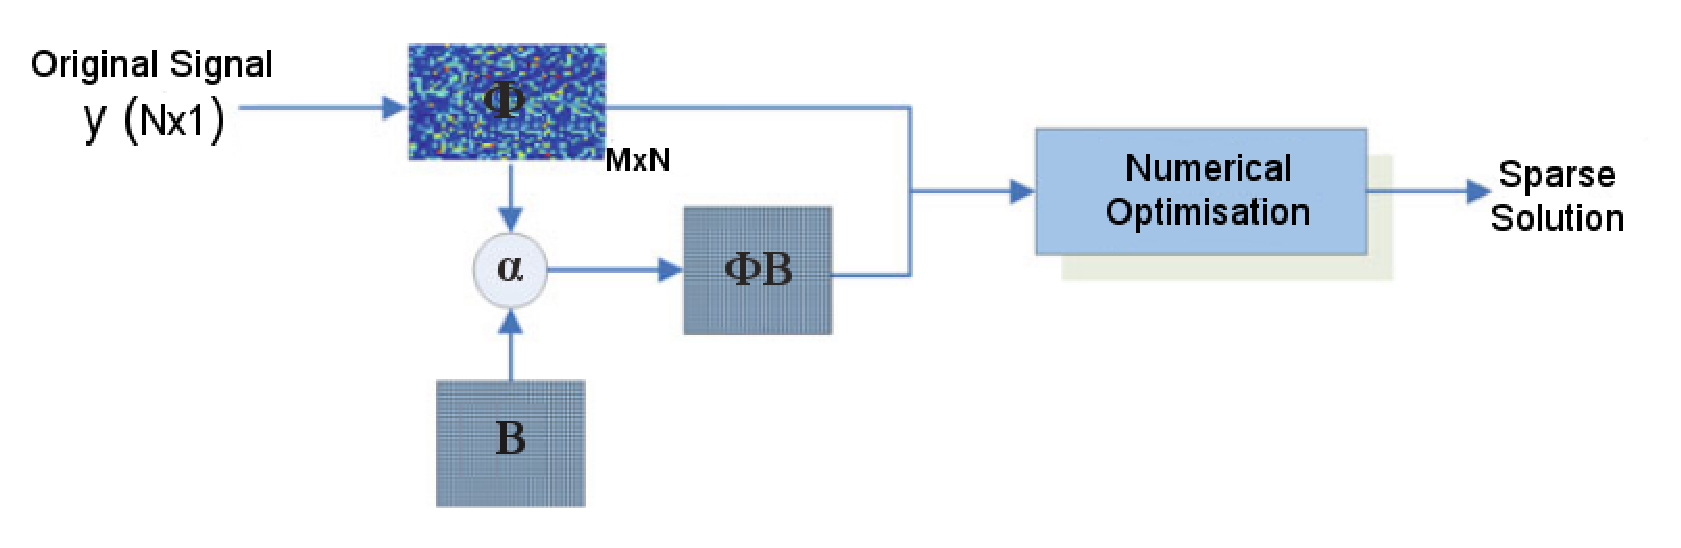
\includegraphics[width=\textwidth]{images/sparse.eps}
\caption[Compressive sensing procedure]{Compressive sensing procedure \cite{compressive}}
\label{fig:compressive}
\end{figure}










\clearpage\chapter{Related Work}

The importance of video service in the cloud is considerable due to lot amount of video information transferred over networks. Recently, video cloud has become a hot research topic. The compressed video sensing (CVS) and sparse representation is an alternative that is gaining strength thanks to the results of compressive sensing (CS) in fields as image/video reconstruction, image/video super-resolution and image/video compression. For video coding with sparse representation, Shen \emph{et al}. in \cite{motion_cs} propose to perform the motion estimation based in sparse representation. A region $C$ denotes the current block to  be predicted and a region $S$ denotes the neighbour blocks of $C$.  search a good approximation for know pixels in a $S$ region and its sparse representation coefficient is calculated and then keep the same procedure to estimate the unknown pixel value in $C$ region. In this proposal two dictionary are used, $D_S$ for pixel of region $S$ and $D_C$ for pixel of region $C$. Sparse representation is calculated with OMP algorithm and energy of residual on the current block is used as the stopping criteria. In \cite{odl_me}, Sun \emph{et al}. propose a framework for inter-frame video coding using sparse representation with online dictionary learning. The dictionary is training with textured patches of each frame in the video in order to obtain sparse representation for the following frames. Furthermore, the sparse coefficients are quantized and encoded using Huffman entropy encode. A module is added in the encoder for construct the sparse representation and another is added the decoder for reconstruct the image. The framework was compared with H.264 video encoder and  K-SVD dictionary, showing better rate distortion performance but increasing the bit rate the performance gradually decrease. \\

For the other hand, Xiong \emph{et al}. in \cite{sparse_st, 6189245} use sparse representation for up-sampling video frame in low resolution. Key frames are selected as high resolution and the non-key frame are down-sampled in low resolution. High resolution version are recovered  using the learning-based super-resolution reconstruction and all frames of the video are encoded and decoded using H.264 encoder. For reconstruction a set of 2-D sub-dictionary pairs (High Resolution and Low resolution) and a 3-D dictionary pair (High Resolution and Low resolution) are created. First dictionary is trained with primitive frame patches and the second dictionary is trained with interpolated patches combined with the most matched patches in the neighbour training frame using K-SVD algorithm. This proposal shows improvements in coding efficiency in low bit-rate regions compared to H.264 encoder. The figure \ref{fig:spatio-temporal} show the learning framework of sparse spatio-temporal representation for video coding. \\

\begin{figure}[!h]
\centering
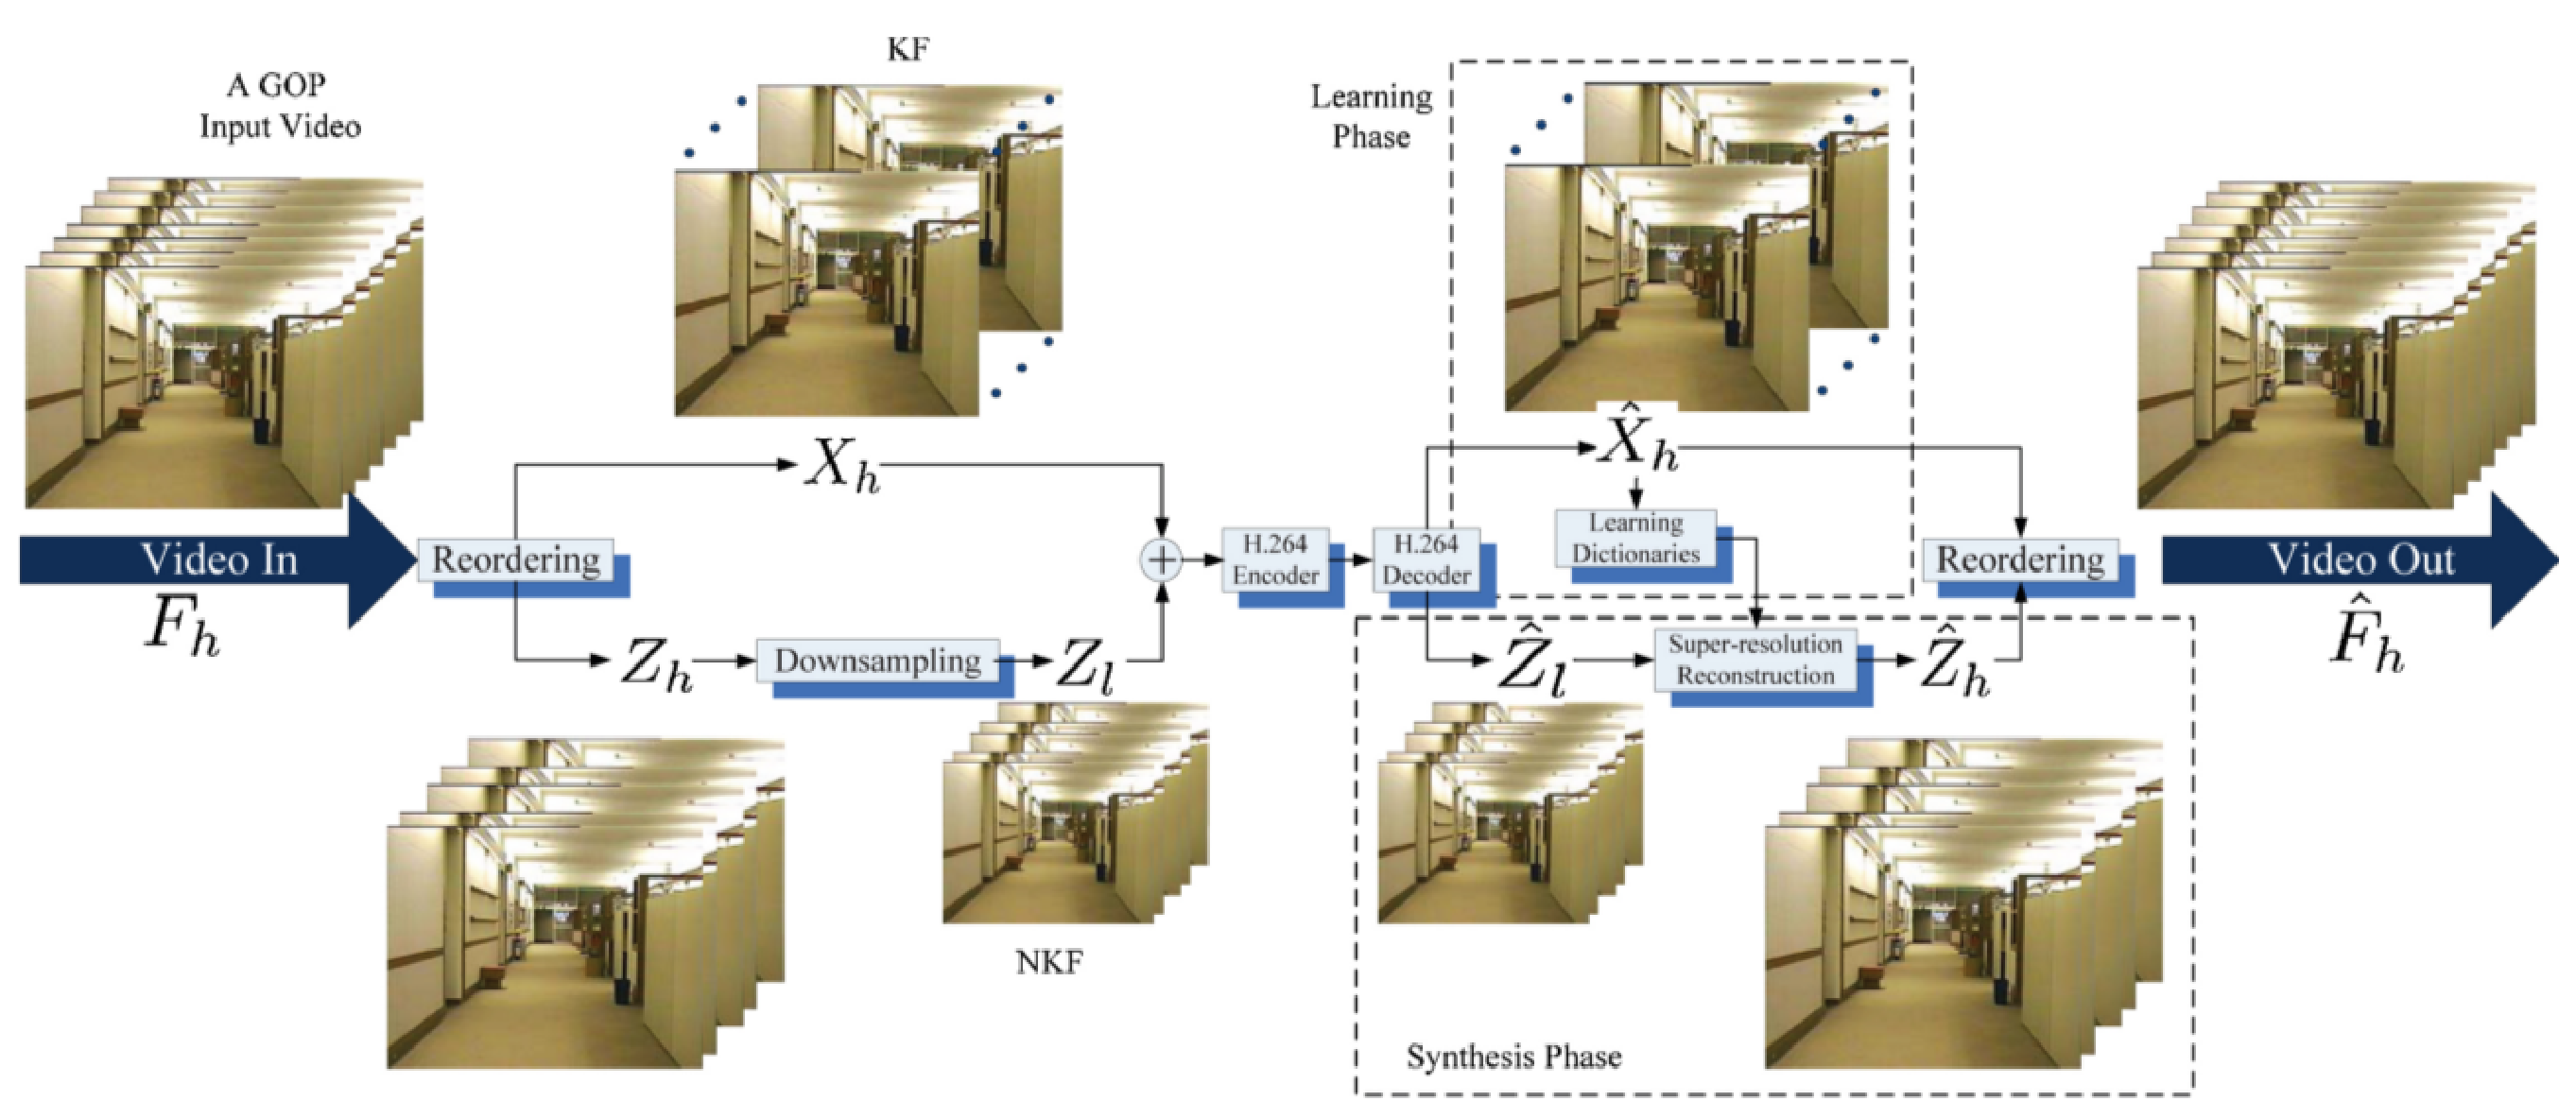
\includegraphics[width=\textwidth]{images/spatio-temporal.eps}
\caption[Learning framework of sparse spatio-temporal representation for video coding]{Learning framework of sparse spatio-temporal representation for video coding \cite{sparse_st}}
\label{fig:spatio-temporal}
\end{figure} 

In the field of compressed video sensing, Azghan \emph{et al}. present in \cite{7076640} a compressive sampling and  multihypothesis reconstruction strategy for video sequences. The video frames are grouped as reference and non-reference. Reference frame is divided into non-overlapping blocks and it are vectorized row-wise, compressively sensed and sent to the  decoder. For each block of the non-reference frames, the corresponding dictionary  is  constructed  by  stacking  (column-wise)  a number  of  vectorized  blocks  of  the  reference frame that are lying inside the search window. At the decoder side, the current block is recovered,  knowing that the current block is sparse in the discrete cosine  transform (DCT) domain using multihypothesis technique (motion estimation task is performed by the decoder instead of encoder). The proposed approach is compared with Multihypotheis Elastinec algorithm \cite{Chen:2015}, obtained  a increasing in PSNR of 1.19 dB on average. In \cite{6984694}  Guo \emph{et al}. propose a new motion estimation method in measurement domain for CVS. This proposal is based on the correlation relationship to  
estimate the measurements of a block in a random unknown position in a frame, taking advantage of measurements of the adjacent non-overlapping blocks. The current block is formulated as a linear combination  of the four non-overlapping blocks using sparse representation. \\
 
In some articles combine the distributed video coding (DVC) with compressing sensing, in a proposal called Distributed Compressed Video Coding (DVCS). DVC avoids the computationally intensive temporal prediction  loop at the encoder, by shifting the exploitation of the temporal redundancy to the decoder \cite{5202822} . For DVCS,  Baig \emph{et al}.propose in \cite{6266276} a codec entirely based on CS. Video frames are divided into key frames and non-key frames and are converted to a column vector for calculate the CS measurements. The calculated measurements are quantized using Gaussian quantization. In the decoder side, each key frame is reconstructed with sparse representation. A dictionary is constructed with CS measurements of key frames available at the decoder for reconstructing the non-key frame based on the correlation between its CS measurements and the dictionary. In \cite{6245804} Yu \emph{et al}. propose a multiple description distributed compressed video sensing. In the multiple description, the video sequence is split into two subsequences (two   descriptions) and compressed with almost the same quality  but  transmitted  over  two  different channels, when all descriptions are received, the central decoder will work to provide  the  best  quality  reconstruction  of  the  video  sequence. At the encoder, the original video sequence is split into key-frame followed by some CS frames and all are compressed by CS method generating two descriptions. The strong  correlation among frames allows that measurement rate of CS-frames can be lower than that of key-frames. Additionally the complexity is reduce using block-level CS. At the decoder, key-frames are recovered by simply applying the block-level CS reconstruction, while for the CS-frames, the CS process is improved by a motion estimation. If all descriptions are received, the decoder central can structure CS frames by searching temporal neighbouring blocks from previously recovered adjacent key-frames using more sparse domains for reconstruction taking advantage of the temporal correlation that exists in the video signal. \\

In the case of cloud-based proposal using CS, Wang \emph{et al}. in \cite{6694139} propose a cloud-based compressive sensing video communication system. The system proposed mainly includes video senders, cloud platform and receivers. The encoder receives the raw samples and generates compressed video frames with CS using block Hadamard of 32 $times$ 32 for construct the dictionary. Video sequence are divided in $I$ frame which are directly compressed and $P$ frame which are encoded by utilizing the temporal redundancy between  adjacent frames. $I$ frame are taken as image reference frame, while $P$ frames are constructed by taking CS scheme of algebraic difference with its closest $I$ frame represented by a vector. For combating the data loss in wireless networks, a CS erasure code (CSEC) adaptive based on bit error rate is proposed. Adaptive error detecting schemes are used in different channel conditions, and  CSEC is combined to compensate for the quality degradation resulted from channel error. The CS-reconstructed video is transcoded to H.264-encoded video streams in the cloud platform and finally transmitted to the receiver. \\

\begin{figure}[!h]
\centering
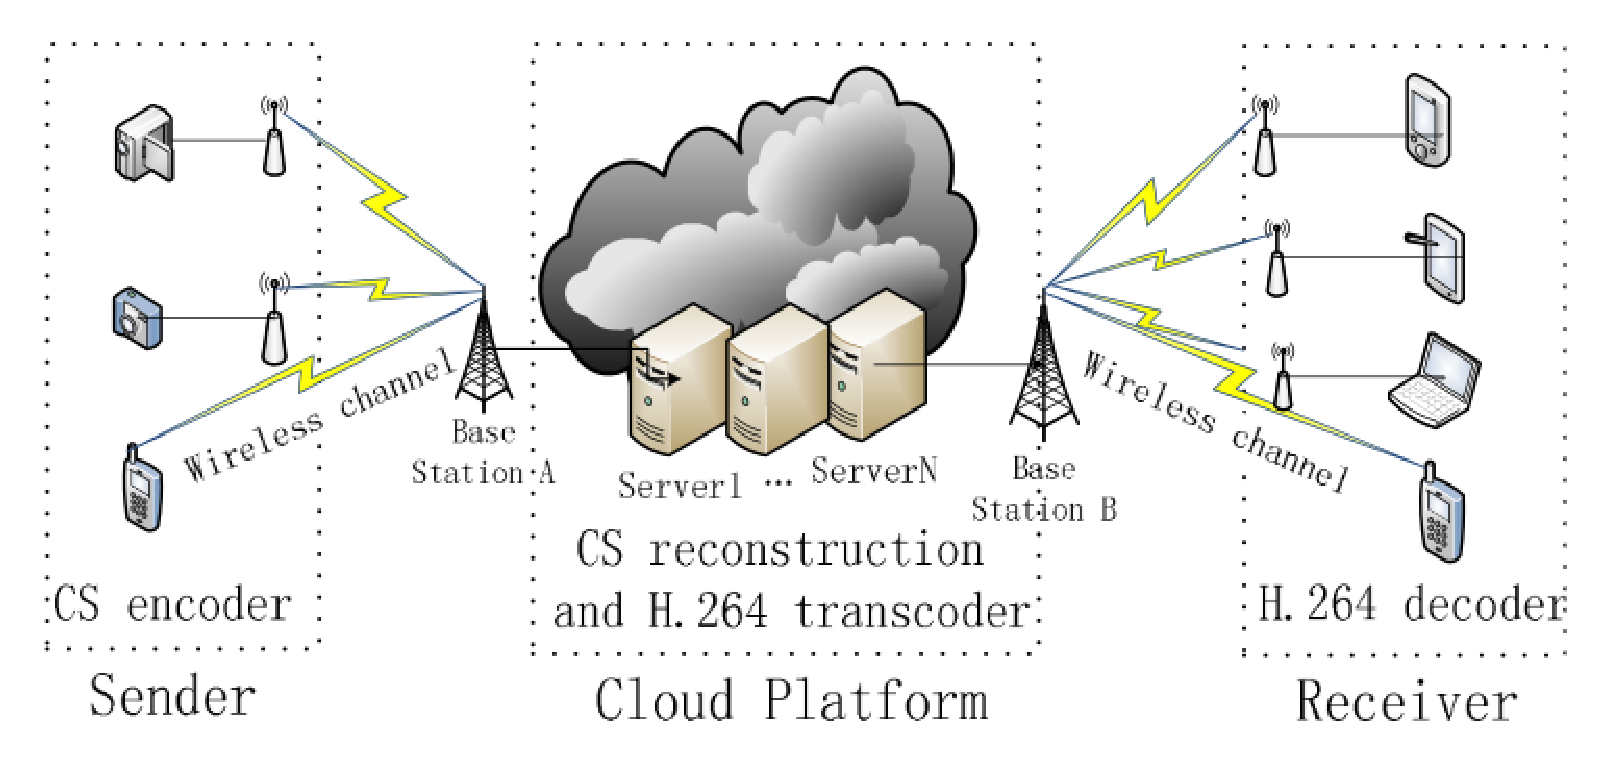
\includegraphics[width=0.6\textwidth]{images/cloud-based.eps}
\caption[Cloud-based compressive sensing video transmission system]{Cloud-based compressive sensing video transmission system \cite{6694139}}
\label{fig:cloud-based}
\end{figure} 
\clearpage\chapter{Proposed Approach}

%This chapter present a general description of the proposal.
The project addresses the high requirements in bit rate for representing HD video content specifically for transmission through the cloud. For solving this problem, is proposed to use the techniques of compressive sensing in video coding and the elements of fog computing. The proposed approach have two main components:
\begin{description}
\item[encoder:] this component involves the calculus of sparse vectors for representing the video frames.
\item[decoder:] this component involves the reconstruction of the video frames based on the sparse vectors generate by the encoder.
\end{description}

The first step is the training of the dictionary. This dictionary is constructed based on a learning algorithm and can be trained in real-time or can be trained offline and preloaded. Generally, the algorithms trained using patches of video frames; depending on the algorithm and needs, the patches are taken from the video original to encode or from predefined video samples. This consideration should be evaluated in the initial part of the project. \\

Once the dictionary is built, the sparse representation for frames of video sequence are calculated. Each video frame is transmitted to the encoder and in the encoder are constructed the sparse $\boldsymbol{\alpha}$ vector for sparse representation. For this, the values of luminance of the video frame are vectorized in $\boldsymbol{y}$ and, with dictionary $\boldsymbol{D}$, is calculated the vector $\boldsymbol{\alpha}$ that represent $\boldsymbol{y}$ through a lineal combination. The main idea of sparse representation is that vector $\boldsymbol{\alpha}$ contains many zero values as is presented in the Fig. \ref{fig:proposed_sparse}. \\

\begin{figure}[!h]
\centering
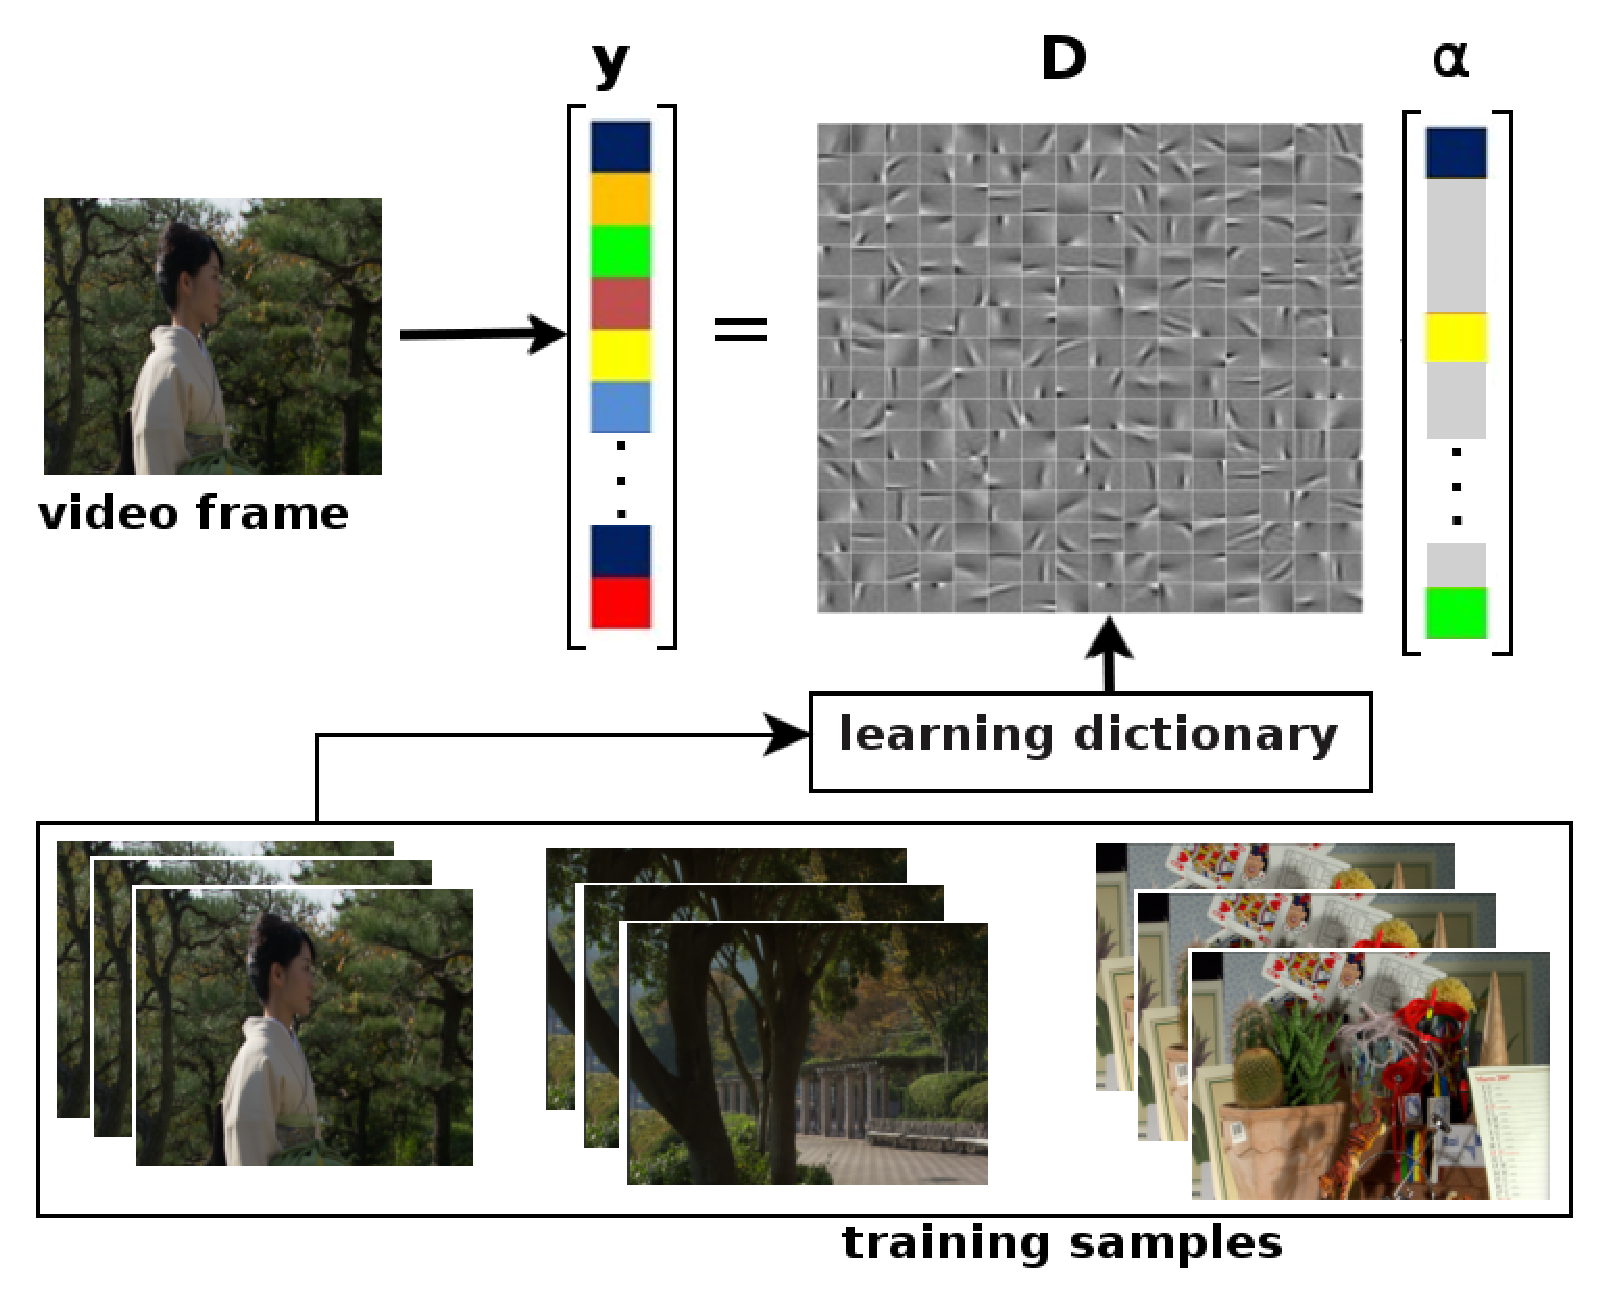
\includegraphics[width=0.45\textwidth]{images/proposed_sparse.eps}
\caption{Sparse representation for video frame}
\label{fig:proposed_sparse}
\end{figure}

The calculated sparse $\alpha$ vector and the dictionary are compressed for reducing the bit for transferring easily. All encoder process is performed in the fog network. In this case, the encoder is implemented using the virtualisation technologies in the edge of the network, with the purpose of reduce the latency compared to the cloud. \\

The information is transferred to the decoder that receives the compressed dictionary $\boldsymbol{D}$ and the sparse vectors $\boldsymbol{\alpha}$,  for decompressing and reconstructing the video frames $\boldsymbol{y}$. The decoder is localised in the end-user.

For the evaluation of coding efficiency are used the Peak Signal-Noise Ratio (PSNR) to evaluated the video quality and the Kbits per second to evaluate the bit rate.
 


\clearpage\chapter{Methodology}


\section{Expected Results}


\section{Budget}


\clearpage\include{Chapters/Bibliography}

\end{document}
